\documentclass{foils}

%\newfont{\cmrhuge}{cmr17 at 160.8pt}
\newfont{\cmrhuge}{cmss17 at 160.8pt}
%\newfont{\cmrhuge2}{cmss17 at 100.8pt}

\topmargin=-65pt
\textheight=7in
\textwidth=10.5in
%%\headsep=.25in
%%\headheight=0in
\oddsidemargin=-.75in
\evensidemargin=-.75in
\usepackage{color}
\usepackage{epsfig}
\usepackage{graphicx}
\special{header=gradient.h}

\newcommand{\newcolor}[3]{\definecolor{#1}{#2}{#3}}

%%%% text color definitions %%%%
%%\newcolor{textcolor}{rgb}{0,0,0}
%%\newcolor{titlecolor}{rgb}{0,0,.5}
%%\newcolor{headingcolor}{rgb}{.5,0,0}
%%\newcolor{bullet1color}{rgb}{0,0,.5}
%%\newcolor{bullet2color}{rgb}{0,.5,0}
%%\newcolor{bullet3color}{rgb}{.5,.5,.5}

%%%% redefine colors for blue background %%%%
\newcolor{textcolor}{rgb}{.9,.9,.9}
\newcolor{titlecolor}{rgb}{0.0,.14,.33}
\newcolor{headingcolor}{rgb}{1,.5,.1}
\newcolor{bullet1color}{rgb}{.9,.9,.3}
\newcolor{bullet2color}{rgb}{0,.7,0}
\newcolor{bullet3color}{rgb}{.7,.7,.7}

\newcommand{\myfig}[2]{
\begin{figure}[h]
\color{textcolor}
\centerline{\includegraphics{figs/#1.eps}}
\caption{#2}
\label{fig:#1}
\end{figure}
}

%%%%% modify these %%%%%
\newcommand{\talktitle}{\color{titlecolor}{\cmrhuge Codegen}}
\newcommand{\talkdate}{\date{June 2000}}
\MyLogo{\color{textcolor} 06/00} %%also date of talk
%%%%%%%%%%%%%%%%%%%%%%%%


\newsavebox{\gradient}
\sbox{\gradient}{
        \includegraphics[width=15in,height=6.75in]{gradient.ps}
        }

\leftheader{
        \vbox{
        \vspace*{135pt}
        \hskip -34.5pt
        \usebox{\gradient}
        }
}
\rightfooter{\color{textcolor} \arabic{page}/\pageref{'eof'}}
\LogoOff
\newcommand{\nextfoil}{ \foilhead[-.6in]}
%{ \talktitle } }
\newcommand{\ctitle}[1]{\begin{center}{\color{headingcolor}\Huge #1}\end{center}
}
%\newcommand{\nfoil}[1]{\nextfoil\ctitle{#1}}
\newcommand{\nfoil}[1]{\foilhead[-.6in]{ \ctitle{#1}\vspace*{60pt}}}
\renewcommand{\theenumi}{\color{bullet2color}\arabic{enumi}}
\renewcommand{\theenumii}{\color{bullet2color}\arabic{enumii}}
\renewcommand{\theenumiii}{\color{bullet2color}\arabic{enumiii}}
\renewcommand{\labelitemi}{\color{bullet1color}$\bullet$}
\renewcommand{\labelitemii}{\color{bullet2color}--}
\renewcommand{\labelitemiii}{\color{bullet3color}$\triangleright$}

\begin{document}

\color{textcolor}
\title{
\hskip -84pt
\vbox{
        \vspace*{70pt}
        \usebox{\gradient}
        \vspace{-7.5in}
}
\\
\talktitle\\*[1 in]
}
\author{
\color{headingcolor}\LARGE Caroline Dahll\"{o}f \\ caro@rhythm.com \\*[.5 in]}
\talkdate
\maketitle

{\Large
\nfoil{Overview}
%%only the first foil needs to do \LogoOn
\LogoOn
\begin{itemize}
\item What are the problems? 
\item How we solved it?
\item Assumptions we made
\item Generic Image Language
\item Codegen
\item Limitations
\end{itemize}

\nfoil{What are the problems?}
\begin{itemize}
\item Different data types and color models
\item Promotion
\item Overflow 
\end{itemize}


\nfoil{How we solve it?}
\begin{itemize}
\item Generic Image Language (GIL) 
\item Codegen
\end{itemize}

\nfoil{Assumptions we made}
\begin{itemize}
\item Channel data are pointers 
\item Independent code is left outside GIL blocks  
\end{itemize}

\nfoil{Overview}
\begin{itemize}
\item Generic Image Language
\begin{itemize}
\item Definition
\item Example
\item Declaration Block
\item Initialization Block
\item Code Block
\item DT Macros
\end{itemize}
\end{itemize}

\nfoil{Generic Image Language}
\begin{itemize}
\item Independent of data type and color model 
\item Uses macros for dependent operations
\item Easy to read and write 
\end{itemize}

\nfoil{Example}
\begin{flushleft}
\tt
\small
GENERIC\_IMAGE\_DECL\_BEGIN\\
Pixel dest(color,alpha,has\_alpha);\\
Pixel src1(color,alpha,has\_alpha);\\
Pixel src2(color,alpha,has\_alpha);\\
GENERIC\_IMAGE\_DECL\_END\\*[0.5cm]
GENERIC\_IMAGE\_IMAGE\_DATA\_INIT\\*[0.5cm]
GENERIC\_IMAGE\_CODE\_BEGIN\\
dest\_color = CHANNEL\_CLAMP((Promote)src1\_color + src2\_color);\\
if (dest\_has\_alpha)\\
\hspace*{.4cm} \{\\
\hspace*{.8cm} if (src1\_has\_alpha \&\& src2\_has\_alpha)\\
\hspace*{1.2cm} \{\\
\hspace*{1.6cm} dest\_alpha = CHANNEL\_CLAMP ((Promote)src1\_alpha + src2\_alpha);\\
\hspace*{1.2cm} \}\\
\hspace*{.8cm} else if (src1\_has\_alpha)\\
\hspace*{1.2cm} \{\\
\hspace*{1.6cm} dest\_alpha = WP;\\
\hspace*{1.2cm} \}\\
\hspace*{.8cm} else if (src2\_has\_alpha)\\
\hspace*{1.2cm} \{\\
\hspace*{1.6cm} dest\_alpha = WP;\\
\hspace*{1.2cm} \}\\
\hspace*{.8cm} \}\\
dX (dest,1);\\
dX (src1,1);\\
dX (src2,1);\\
GENERIC\_IMAGE\_BLOCK\_END\\
\end{flushleft}


\nfoil{Declaration Block}
\begin{itemize}
\item GENERIC\_IMAGE\_DECL\_BEGIN\\ ... \\GENERIC\_IMAGE\_DECL\_END 
\item Pixel name (color,alpha,has\_alpha)
\item Channel name 
\item int, float  
\end{itemize}

\nfoil{Initialization Block}
\begin{itemize}
\item GENERIC\_IMAGE\_IMAGE\_DATA\_INIT
\item Sets Pixel variable equal to their data value 
\end{itemize}

\nfoil{Code Block}
\begin{itemize}
\item GENERIC\_IMAGE\_CODE\_BEGIN\\ ... \\GENERIC\_IMAGE\_CODE\_END
\item Pixel (name/name\_color/name\_alpha)
\item DT Macros 
\item Promotion  
\end{itemize}

\nfoil{DT Macros}
\begin{itemize}
\item Data types
\begin{itemize}
\item DATATYPE
\item PROMOTE\_TYPE
\item SIGNED\_PROMOTE\_TYPE
\end{itemize}
\item Channel Constants
\begin{itemize}
\item WP
\item WP\_NORM
\item CHANNEL\_MIN
\item CHANNEL\_MAX
\end{itemize}
\item Channel Operations
\begin{itemize}
\item CHANNEL\_CLAMP (x)
\item WP\_CLAMP (x)
\item CHANNEL\_MULT (x,y)
\item CHANNEL\_ROUND (x)
\end{itemize}
\item Iterator operations
\begin{itemize}
\item dX (Pixel,x) 
\item dY (Pixel,x) 
\end{itemize}
\item PRINT (x)
\item EXTERNAL\_INIT (x)
\end{itemize}

\nfoil{Overview}
\begin{itemize}
\item Codegen
\begin{itemize}
\item Definition
\item How to run Codegen
\item Color Channel names
\item Channel data file
\item Example
\item Creating dependent code
\item Implementation details
\end{itemize}
\end{itemize}

\nfoil{Codegen}
\begin{itemize}
\item Parses Generic Image Language
\item Creates data type and color model dependent code
\item Independent of data type and color model 
\end{itemize}

\nfoil{How to run Codegen}
\begin{flushleft}
\tt
codegen --channel-names COLOR\_CHANNEL\_NAMES\\  
\hspace{4em}--channel-data-file CHANNEL\_DATA\_FILE 
\end{flushleft}

\nfoil{Color Channel names}
\begin{itemize}
\item Separated by ','
\item Always adds an alpha channel
\end{itemize}

\nfoil{Channel data file}
\begin{itemize}
\item Contains definition for DT Macros
\item Example of 16bit 4K WP 
\tt
\small 
\begin{tabbing}
DT\_MACROS\_BEGIN\\ 
\hspace*{0.5cm}\=DATATYPE \=\hspace{7cm}\= guint16 \\ 
\>PROMOTE\_TYPE \>\> (guint32)\\  
\>SIGNED\_PROMOTE\_TYPE \>\> (gint32)\\  
\>WP \>\> 4095UL\\ 
\>WP\_NORM \>\> (1/4095.0)\\ 
\>CHANNEL\_MIN \>\> 0\\ 
\>CHANNEL\_MAX \>\> 65535\\ 
\>ZERO \>\> 0UL\\ 
\>CHANNEL\_CLAMP (x) \>\> CLAMP (x,0,65535)\\ 
\>WP\_CLAMP (x) \>\> CLAMP (x,0,4095)\\ 
\>CHANNEL\_MULT (x,y) \>\> (x * y)/4095UL\\ 
\>CHANNEL\_ROUND (x) \>\> ROUND (x)\\ 
\>PRINT (x) \>\> printf (" \%uh", x)\\ 
\>EXTERNAL\_INIT (x) \>\> x.u16\_k\\ 
DT\_MACROS\_END
\end{tabbing}
\end{itemize}


\nfoil{Example}
\begin{flushleft}
\tt
\small
guint16 *dest\_data[4];\\
gboolean dest\_has\_alpha;\\
guint16 *dest\_red, *dest\_green, *dest\_blue, *dest\_alpha=NULL;\\
guint16 *src1\_data[4];\\
gboolean src1\_has\_alpha;\\
guint16 *src1\_red, *src1\_green, *src1\_blue, *src1\_alpha=NULL;\\
guint16 *src2\_data[4];\\
gboolean src2\_has\_alpha;\\
guint16 *src2\_red, *src2\_green, *src2\_blue, *src2\_alpha=NULL;\\*[.5cm]

dest\_red = dest\_data[0];\\
dest\_green = dest\_data[1];\\
dest\_blue = dest\_data[2];\\
if (dest\_has\_alpha)\\
\hspace*{.4cm} dest\_alpha = dest\_data[3];\\*[.5cm]

src1\_red = src1\_data[0];\\
src1\_green = src1\_data[1];\\
src1\_blue = src1\_data[2];\\
if (src1\_has\_alpha)\\
\hspace*{.4cm} src1\_alpha = src1\_data[3];\\*[.5cm]

src2\_red = src2\_data[0];\\
src2\_green = src2\_data[1];\\
src2\_blue = src2\_data[2];\\
if (src2\_has\_alpha)\\
\hspace*{.4cm} src2\_alpha = src2\_data[3];\\*[.5cm]

*dest\_red = CLAMP ((guint32)   *src1\_red + *src2\_red,0,65535);\\*
*dest\_green = CLAMP ((guint32)   *src1\_green + *src2\_green,0,65535);\\*
*dest\_blue = CLAMP ((guint32)   *src1\_blue + *src2\_blue,0,65535);\\*[.5cm] 
if (dest\_has\_alpha)\\
\hspace*{.4cm} \{\\
\hspace*{.8cm} if (src1\_has\_alpha \&\& src2\_has\_alpha)\\
\hspace*{1.2cm} \{\\
\hspace*{1.6cm} *dest\_alpha = CLAMP ((guint32)   *src1\_alpha + *src2\_alpha,0,65535);\\
\hspace*{1.2cm} \}\\
\hspace*{.8cm} else if (src1\_has\_alpha)\\
\hspace*{1.2cm} \{\\
\hspace*{1.6cm} *dest\_alpha = 4095UL;\\
\hspace*{1.2cm} \}\\
\hspace*{.8cm} else if (src2\_has\_alpha)\\
\hspace*{1.2cm} \{\\
\hspace*{1.6cm} *dest\_alpha = 4095UL;\\
\hspace*{1.2cm} \}\\
\hspace*{.4cm} \}\\*[.5cm]
         
dest\_red++;\\
dest\_green++;\\
dest\_blue++;\\
if (dest\_has\_alpha)\\
\hspace*{.4cm} dest\_alpha++;\\*[.5cm]

src1\_red++;\\
src1\_green++;\\
src1\_blue++;\\
if (src1\_has\_alpha)\\
\hspace*{.4cm} src1\_alpha++;\\*[.5cm]

src2\_red++;\\
src2\_green++;\\
src2\_blue++;\\
if (src2\_has\_alpha)\\
\hspace*{.4cm} src2\_alpha++;
\end{flushleft} 

\nfoil{Creating dependent code}
\begin{itemize}
\item Pixel a(color,alpha,has\_alpha)\\
\small {\hspace*{.4cm} guint16 *a\_data[4];\\*[-.5cm]
\hspace*{.4cm} gboolean a\_has\_alpha;\\*[-.5cm]
\hspace*{.4cm} guint16 *a\_red, *a\_green, *a\_blue, *a\_alpha=NULL;}
\Large
\item Channel b;\\
\small {\hspace*{.4cm} guint16 *b;}
\Large
\item PRINT (a);\\
\small {\hspace*{.4cm} printf (" \%uh", *a\_red);\\*[-.5cm]
\hspace*{.4cm} printf (" \%uh", *a\_green);\\*[-.5cm]
\hspace*{.4cm} printf (" \%uh", *a\_blue);\\*[-.5cm]
\hspace*{.4cm} if (a\_has\_alpha)\\*[-.5cm]
\hspace*{.8cm} printf (" \%uh", *a\_alpha);}
\Large
\item a = b * a;\\
\small {\hspace*{.4cm} *a\_red = (b * *a\_red)/4095UL;\\*[-.5cm]
\hspace*{.4cm} *a\_green = (b * *a\_green)/4095UL;\\*[-.5cm]
\hspace*{.4cm} *a\_blue = (b * *a\_blue)/4095UL;\\*[-.5cm]
\hspace*{.4cm} if (a\_has\_alpha)\\*[-.5cm]
\hspace*{.8cm} *a\_alpha = (b * *a\_alpha)/4095UL;}
\Large
\item a = EXTERNAL\_VARIABLE (v);\\
\small {\hspace*{.4cm} *a\_red = v[0].u16\_4k;\\*[-.5cm]
\hspace*{.4cm} *a\_green = v[1].u16\_4k;\\*[-.5cm]
\hspace*{.4cm} *a\_blue = v[2].u16\_4k;\\*[-.5cm]
\hspace*{.4cm} if (d\_has\_alpha)\\*[-.5cm]
\hspace*{.8cm} *a\_alpha = v[3].u16\_4k;} 
\Large
\item a = a / 5.0;\\
\small {\hspace*{.4cm} a\_red = ROUND (*a\_red / 5.0);\\*[-.5cm]
\hspace*{.4cm} a\_green = ROUND (*a\_green / 5.0);\\*[-.5cm]
\hspace*{.4cm} a\_blue = ROUND (*a\_blue / 5.0);\\*[-.5cm]
\hspace*{.4cm} a\_alpha = ROUND (*a\_alpha / 5.0);} 
\Large
\item a\_color = CHANNEL\_CLAMP (a\_color + a\_color);\\
\small {\hspace*{.4cm} *a\_red = CLAMP (*a\_red + *a\_red,0,255);\\*[-.5cm]
\hspace*{.4cm} *a\_green = CLAMP (*a\_green + *a\_green,0,255);\\*[-.5cm]
\hspace*{.4cm} *a\_blue = CLAMP (*a\_blue + *a\_blue,0,255);}
\Large
\item a\_alpha = WP - ((WP - a\_alpha) * (WP - a\_alpha));\\
\small {\hspace*{.4cm} *a\_alpha = 4095UL - (((4095UL - *a\_alpha) * (4095UL - *a\_alpha))/4095UL);}
\Large 
\end{itemize}

\nfoil{Implementation details}
\begin{itemize}
\item Written in Flex \& Bison 
\end{itemize}

\nfoil{Flex}
\begin{figure}[tp]
\centering
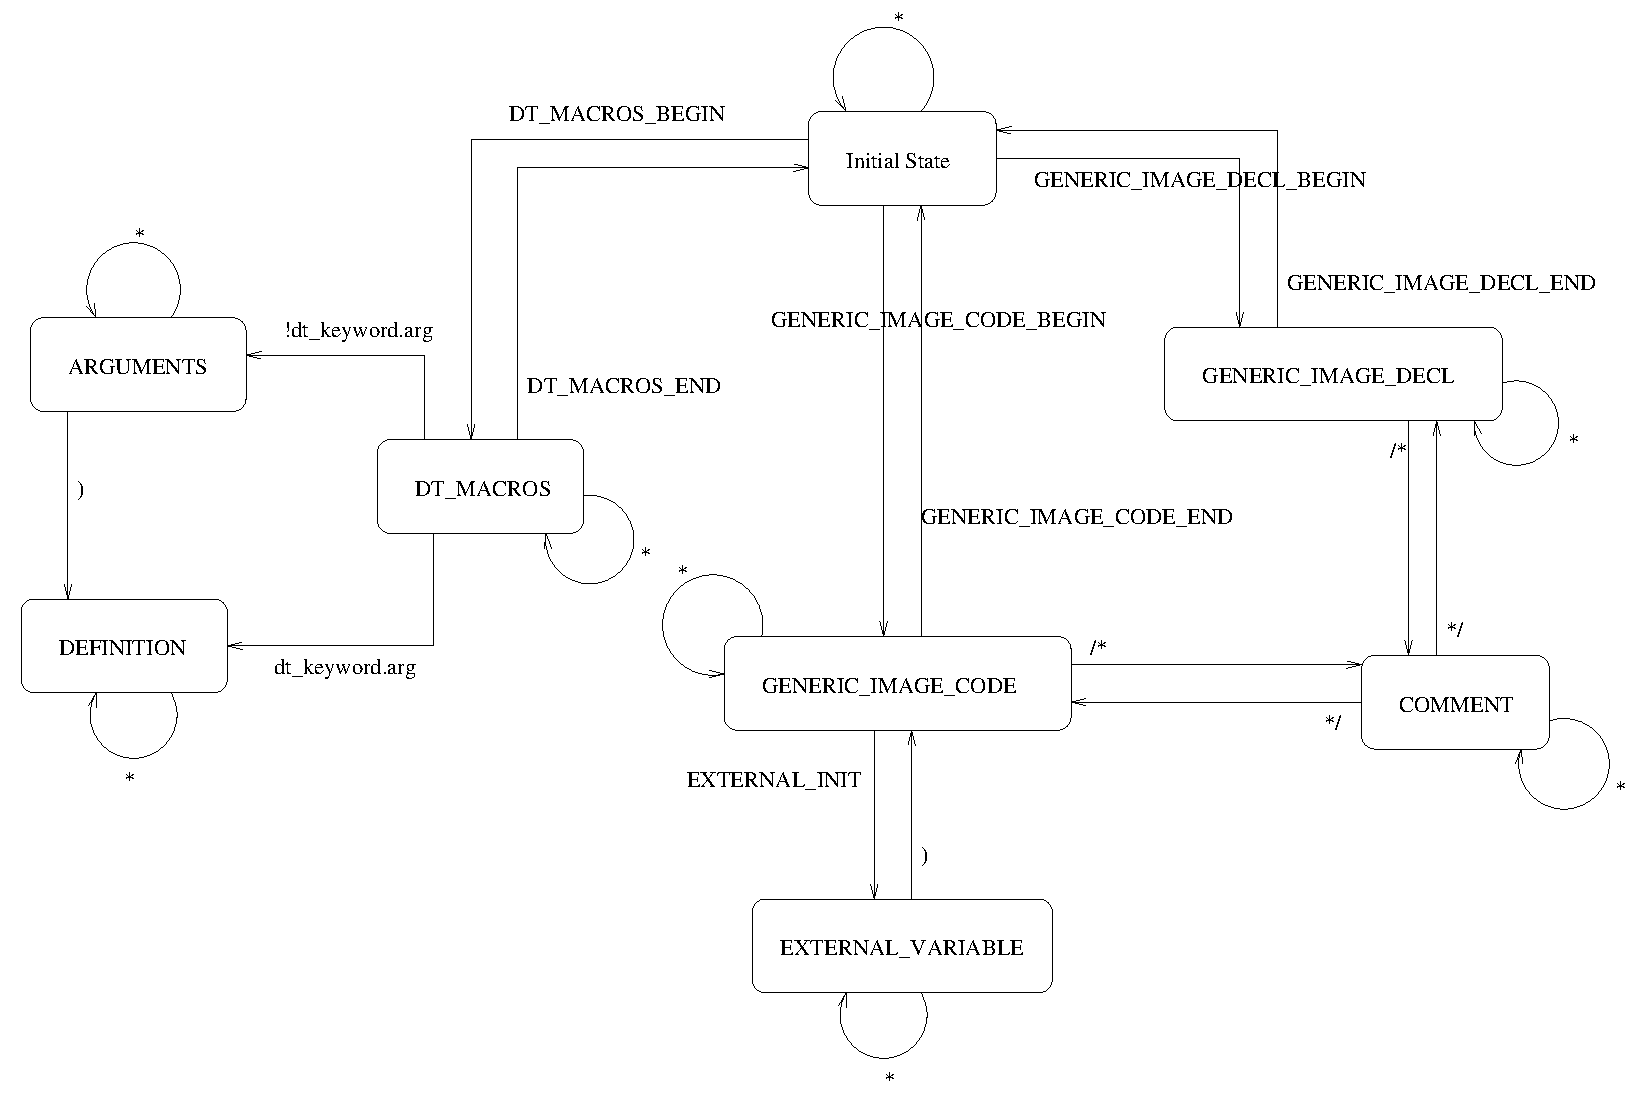
\psfig{file=./file.ps, width=8in}
\end{figure}

\nfoil{Bison} 
\begin{itemize}
\item Defines GIL grammar
\item Expands Pixel to channels
\item Converts DT Macros into specific code 
\end{itemize}

\nfoil{Limitations}
\begin{itemize}
\item Channels of different ranges 
\end{itemize}

\nfoil{More Information}
\begin{itemize}
\item Codegen, GIL and GEGL 
\begin{itemize}
\small
\item http://film.gimp.org/geglCodegen.html
\item http://www.mindspring.com/\~calvinw/genericChannelData.html
\item http://www.mindspring.com/\~calvinw/genericImageLanguage.html
\item http://www.mindspring.com/\~calvinw/geglClasses.html
\end{itemize}
\item The 16 bit GIMP
\begin{itemize}
\small
\item http://film.gimp.org/
\end{itemize}
\item The GIMP's SIGGRAPH meeting
\begin{itemize}
\small
\item http://siggraph.gimp.org 
\end{itemize}
\end{itemize}

\nfoil{Thanks}
\begin{flushleft}
Many thanks to Calvin Williamson, The GIMP community, Rhythm \& Hues, and a special thanks to our sponsors the Free Software Foundation, the Chaos Computer Club, and O'Reilly Germany 
\end{flushleft}

%%End of file label to make numbering work
\label{'eof'}
\end{document}


